\documentclass[12pt]{article}         
\usepackage{fullpage}
\usepackage[shortlabels]{enumitem}
\usepackage{amsmath}
\usepackage{amsfonts}
\usepackage{graphicx}
\graphicspath{ {./images/} }

%\usepackage{amsmath}
%\usepackage{amssymb}
%\usepackage{enumitem}

\title{CS250 Homework $\#$5}
\author{Sean O'Dea \footnote{Collaborated with Nobody.}}

\begin{document}
\maketitle

\section*{\textbf{1: P9.5.2} [12 pts]}
Suppose that a directed acyclic graph has maximum path length $d$ and that no node has more than $b$ neighbors. What is the largest number of node visits that could occur in a depth-first search of this graph? Show an example of such a graph that has only $bd + 1$ nodes and has the maximum number of node visits.


\subsection*{\textbf{Solution:}}
The largest number of node visits would be a scenario where the depth first search occurs on a directed acyclic graph with one root such that it forms a full rooted tree. In this case the DFS will reach every node of the graph if it starts at the root. The number of neighbors $b$ is analogous to the degree of the tree $k$ and the maximum path $d$ is analogous to the depth $d$ of the tree. This means we can represent the max number of node visits based on $b$ and $d$ using the formula for the max number of nodes in a tree based on degree and depth from HW4.
\[ \text{Max} = \dfrac{b^{d+1} - 1}{b-1} \text{, Assuming } b > 1 \] 

\noindent
If we consider the graph with $b=2$ and $d=1$ that constructs a rooted tree, we'll get:
\begin{figure}[h]
    \centering
    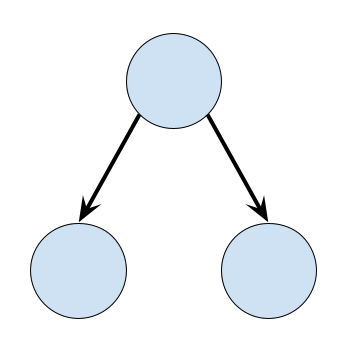
\includegraphics[width=0.25\linewidth]{graph.png}
\end{figure}

\noindent
This graph contains $(2)(1) + 1 = 3$ nodes and if we perform a DFS from the root all nodes will be reached. Note that,
\[ \dfrac{(2)^{(1)+1} - 1}{(2)-1} = \dfrac{3}{1} = 3\]
The formula for max node visits is satisfied.

\newpage
\section*{\textbf{2: P9.6.8} [12 pts]}
Let $G$ be an undirected graph with $n$ nodes that contains two nodes $s$ and $t$, such that the shortest path from $s$ to $t$ has more than $n/2$ edges. Prove that there exists a node $u$, different from $s$ and $t$, such that every path from $s$ to $t$ passes through $u$.


\subsection*{\textbf{Solution:}}
We can prove this by considering three cases. \\

For the first case, assume $s$ and $t$ are in a cycle with each other. This would suggest that $u$ doesn't have to exist because there would exist a path around the cycle from $t$ to $s$ or vice versa that doesn't contain $u$ (because $G$ is undirected). 

If $s$ and $t$ can exist in a cycle together, it would suggest our premise is false so let's determine if we can satisfy the $n/2$ property with a cycle. To maximize the potential for the shortest path from $s$ to $t$ to have more than $n/2$ edges, it would make sense for us to minimize $n$. This means we'll assume the only nodes in the graph exist in this cycle to give the best chance to satisfy the property. We now know that there exists $n$ nodes and $n$ edges in our cycle. Again to attempt to satisfy our property let's attempt to place these nodes as far away from each other in the cycle as possible. This would mean there exists $n/2$ edges at most in either direction when going from $s$ to $t$ or vice versa. If we try to increase this on one side of the cycle, the number of edges will decrease on the other side now making that side the shorter path and still under $n/2$ edges.

From this we can conclude that $s$ and $t$ \textit{cannot} exist in a cycle together while satisfying our properties because the shortest path between them can be at most $n/2$ edges. This means our premise has not been disproven by this case for the reasoning above because it is not possible.\\

For the second case, now assume neither $s$ nor $t$ exist in any cycles. Like before, having more nodes makes it more difficult to satify the $n/2$ property so we'll minimize the number of nodes to $s$, $t$, and the nodes that exist on the paths between these two. Because $s$ and $t$ do not exist in any cycles independently, there must only exist one path between them (again because $G$ is undirected). If there exists only one path between the two nodes, the only permutation we can draw where there doesn't exist a node $u$ between them is if the only nodes in the graph are $s$ and $t$ connected by an edge. In this case there's 2 nodes total, and the shortest path between them is of length 1 which is not greater than $n/2$ so the property is not satisfied. In all other cases there is a node $u$ on the single path between $s$ and $t$.

From this we can conclude that all permutations of $G$ where $s$ and $t$ don't exist in any cycles must have a node $u$ such that all the above properties are satisfied.\\

For the third case, assume either $s$ or $t$ or both exist in independent cycles (as in either cycle does not contain both $s$ and $t$, but only one of them). Let's also assume our $n/2$ property is already satisfied for the shortest path between $s$ and $t$. If at least one of the two nodes exists in a cycle that does not contain the other, this implies there may be multiple paths that do not contain $u$. Let's say $s$ is in a cycle and $t$ is not. We know $t$ must exist outside of the cycle and there exists a path from $t$ to $s$. Because $t$ does not form its own cycle with $s$, it must connect to the original cycle at only one place. From this we can conclude that the node at this connection can be $u$ because the paths from $s$ to $t$ can only cross through this one connection.

Now considering if both $s$ and $t$ are in independent cycles, we can use a very similar logic. $s$ and $t$ must not be part of a cycle together so these two independent cycles must connect at only one edge. Again we can consider the node at this edge $u$ because all paths must cross through it.\\

We have now shown in all three cases that either the properties of the premise cannot be met or if they can be met there must exist a node $u$ such that all paths from $s$ to $t$ pass through it.


\newpage
\section*{\textbf{3: P9.8.8} [10 pts]}
Here is a single-step distance matrix for a weighted directed graph (shown in Figure 9-16) that indicates driving times among six locations in Massachusetts during Friday rush hour. The locations are Amherst (Amh), Hadley (Had), North Amherst (NAm), North Hadley (NHa), Northampton (Ntn), and Sunderland (Sun). An entry of \texttt{--} in the table indicates that there is no edge. (You may ignore the numbers next to each town name in Figure 9-16 – these will be used in Problem 9.9.7.)

\begin{figure}[h]
    \centering
    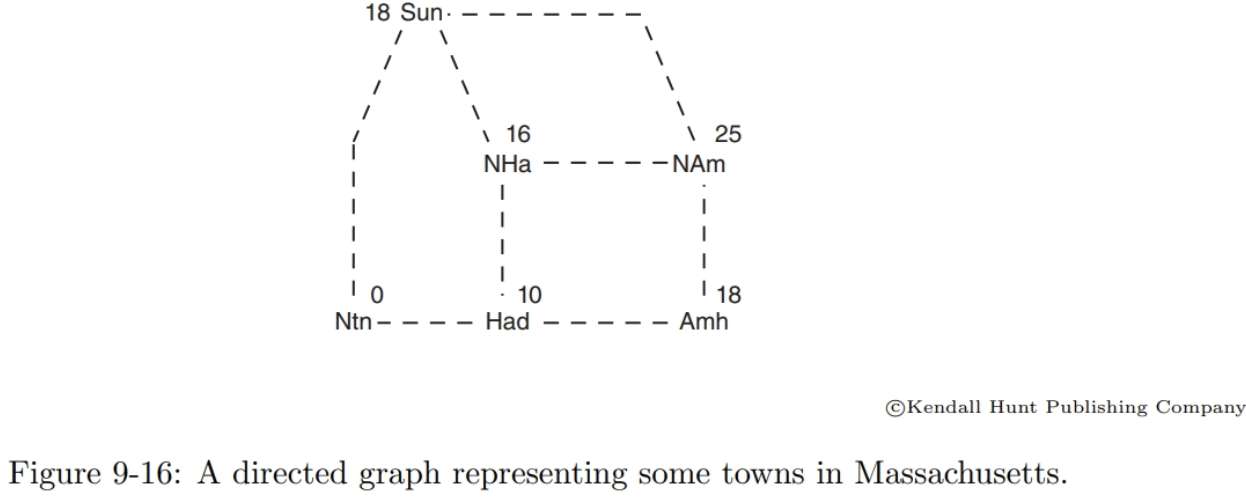
\includegraphics[width=0.5\linewidth]{Fig_9-16.png}
\end{figure}

\begin{verbatim}
    Amh Had NAm NHa Ntn Sun
Amh   0  15  15  --  --  --
Had  12   0  --   8  30  --
NAm  19  --   0  10  --  14
NHa  --  10   9   0  --  12
Ntn  --  15  --  --   0  20
Sun  --  --  11  12  22   0

\end{verbatim}

Use a uniform-cost search (with a closed list, recognizing previously seen nodes) to determine the fastest driving route and shortest-path distance from North Amherst to Northampton.

\subsection*{\textbf{Solution:}}
For this search we'll use a priority queue with elements of the type (location, distance, parent). Also assume the algorithm automatically ignores going directly backwards on the path it took to a node, as this will always take longer. It will also check if a location is already on the queue and compare the existing driving time with the current one. If the existing driving time is shorter, the new entry will be ignored. Same goes if the node reached is already on the closed list. This will be noted below.

\begin{verbatim}
(NAm, 0, NAm) goes on
(NAm, 0, NAm) comes off
(Sun, 14, NAm), (NHa, 10, NAm), (Amh, 19, NAm) go on
(NHa, 10, NAm) comes off; (Had, 20, NHa) goes on; (Sun, 24, NHa) is ignored
(Sun, 14, NAm) comes off; (Ntn, 36, Sun) goes on; (NHa, 26, Sun) is ignored
(Amh, 19, NAm) comes off; (Had, 34, Amh) is ignored
(Had, 20, NHa) comes off; (Ntn, 50, Had) and (NHa, 28, Had) are ignored
(Ntn, 36, Sun) comes off; Goal has been reached
\end{verbatim}

The fastest driving route from North Amherst to Northampton is from North Amherst to Sunderland, and Sunderland to Northampton. This will take 36 minutes total.

\newpage
\section*{\textbf{4: P9.8.9} [10 pts]}
Our uniform-cost search is very similar to \textbf{Dijkstra’s Algorithm}, the best-known method of solving the single-source shortest path problem. In one formulation, Dijkstra’s Algorithm keeps an array $D$ indexed by the nodes of the graph, so that $D(x)$ indicates the shortest \textit{so far known} distance from $s$ to $x$. Initially we set $D(s)$ to 0 and $D(x)$ to $\infty$ for all other nodes $x$. Another boolean array classifies each node as “explored” or “unexplored”, with all nodes initially unexplored. \\
A step of the algorithm is as follows: 
\begin{itemize}
    \item Find the unexplored node $x$ with the smallest value of $D(x)$.

    \item  For every edge out of $x$, to node $y$ with cost $c(x, y)$, compute $D(x) + c(x, y)$.

    \item If any of these values are smaller than the corresponding $D(y)$, reset $D(y)$ to the new value.

    \item Mark $x$ as explored.

\end{itemize}
The algorithm ends if a goal node is marked explored, or if $D(x)$ for every unexplored $x$ is $\infty$.

\begin{enumerate}[(a)]
    \item Explain how this algorithm corresponds to a uniform-cost search of the same graph, in particular how each step of one corresponds to a step of the other.

    \item Uniform-cost search uses a priority queue. Explain how a priority queue can be used to improve the running time of Dijkstra’s Algorithm.
\end{enumerate}

\subsection*{\textbf{Solution:}}
\begin{enumerate}[(a)]
    \item The first step of Dijkstra's Algorithm corresponds with polling the priority queue. In doing this we remove an unexplored node $x$ with the smallest distance to it on the queue, minimizing $D(x)$.

		The second step corresponds with adding each of the nodes that can be reached from $x$ to the open priority queue. The total distance to each of them using the current path is then calculated which will be used in the next step.

		The third step corresponds with the decision of the UCS algorithm to add or ignore the newly discovered path to $y$. If the new path is shorter than the existing one in the queue, the existing path can be replaced. Otherwise it can be left out because a shorter path already exists to $y$.

		The fourth step is the same as adding the node $x$ to the closed list.

    \item Our implementation of UCS is faster than Dijkstra's Algorithm because it utilizes a priority queue rather than an array to store the open list. In UCS when we take the next item off the list, it's removed in logarithmic time. This is more efficient than Dijkstra's Algorithm who removes items in \textit{linear} time off of the open list. This is because it must iterate through the array and compare all elements to find the unexplored node with minimum distance to it. This is assuming it's using a basic, unsorted array of course. If it used an array-based implementation of a priority queue heap it could achieve the same performance as our UCS.
\end{enumerate}


\newpage
\section*{\textbf{5: P9.9.7} [12 pts]}
Conduct an $A^*$ search of the weighted directed graph of Problem 9.8.8, with start node North Amherst and goal node Northampton. Use the heuristic function $h$ defined by $h$(Ntn) = 0, $h$(Had) = 10, $h$(NHa) = 16, $h$(Amh) = 18, $h$(Sun) = 18, and $h$(NAm) = 25. (This heuristic represents the time needed to drive to Northampton with no traffic.) Figure 9-16 shows the heuristic value for each node, and the driving times are given in a table in Problem 9.8.8. Has the traffic in the original problem affected the optimal route from North Amherst to Northampton?


\subsection*{\textbf{Solution:}}
This will follow a similar procedure as the solution to P9.8.8 but this time we will use the heuristic values. Our priority queue will now contain elements of the form (location, distance to parent, $h(x)$, parent).

\begin{verbatim}
(NAm, 0, 25, NAm) goes on
(NAm, 0, 25, NAm) comes off; (Amh, 0, 18, NAm), (Sun, 0, 18, NAm) go on
(Amh, 0, 18, NAm) comes off; (Had, 19, 10, Amh) goes on
(Sun, 0, 18, NAm) comes off; (Ntn, 14, 0, Sun), (NHa, 14, 16, Sun) go on
(Ntn, 14, 0, Sun) comes off; Goal has been reached
\end{verbatim}

\noindent
As expected we reach the same conclusion as when we used the UCS. The fastest route with the traffic is from North Amherst to Sunderland then to Northampton which would take 36 minutes. This is 11 minutes longer than the heuristic estimated. 
\\

\noindent
We can't find the optimal route without traffic based on the heuristic information alone. This is because we only know the time it takes from each location, not specifically which edges will take this much time. Based on the information we're given we can't differentiate how long it takes to get to Hadley from North Amherst on either route so we would just have to assume they're the same and thus there would be no optimal route.

\newpage
\section*{\textbf{6: P5.1.6} [12 pts]}
Let $A$ be any finite alphabet. The language $A^{\leq k}$ is defined to be the union $A^0+ A^1+ \ldots + A^k$, the set of all strings over $A$ with length at most $k$. Prove by induction on all naturals $k$ that the languages $(\emptyset ^* + A)^k$ and $A^{\leq k}$ are equal.


\subsection*{\textbf{Solution:}}
Proof by Induction:\\

Base Case: $k=0$, $(\emptyset ^* + A)^0 = \lambda$ and $A^{\leq 0} = \lambda$\\

Inductive Hypothesis: Assume for an arbitrary natural $n$ the following is true:
\[ (\emptyset ^* + A)^n = A^{\leq n} \]

Inductive Step: We now want to prove the above statement for $n = n + 1$.
\[ A^{\leq n+1} = (A^0+ A^1+ \ldots + A^n) + A^{n+1} = A^{\leq n} + A^{n+1} \]
\[ (\emptyset ^* + A)^{n+1} = (\emptyset ^* + A)^n (\emptyset ^* + A) \]
\[ (\emptyset ^* + A)^n (\emptyset ^* + A) = (A^0+ A^1+ \ldots + A^n)(\emptyset ^* + A) \text{ (By IH)} \]
\[ (A^0+ A^1+ \ldots + A^n)(\emptyset ^* + A) = ((A^0+ A^1+ \ldots + A^n)\emptyset ^*) + ((A^0+ A^1+ \ldots + A^n)A) \text{ (By distributive identity)}\]
\[ ((A^0+ A^1+ \ldots + A^n)\emptyset ^*) = (A^0+ A^1+ \ldots + A^n) \text{ (Left)}\]
\[ ((A^0+ A^1+ \ldots + A^n)A) = (A^1 + A^2 + \ldots + A^{n+1}) \text{ (Right)} \]
\[ (A^1 + A^2 + \ldots + A^{n+1}) + (A^0+ A^1+ \ldots + A^n) = (A^0+ A^1+ \ldots + A^n) + A^{n+1} =  A^{\leq n} + A^{n+1} \]
\[ \text{Therefore } (\emptyset ^* + A)^{n+1} = A^{\leq n} + A^{n+1} = A^{\leq n+1} \]
\[ Q.E.D. \]

\newpage
\section*{\textbf{7: P5.2.4} [10 pts]}
Construct a regular expression denoting the language of strings in $\{a, b\}^*$ that have a number of $b$’s that is divisible by 3.


\subsection*{\textbf{Solution:}}
To solve this we can think of all strings in this language as a concatenation of substrings of a certain type. We know the number of $b$'s should be a multiple of 3, so we can say each of these substrings will have 3 $b$'s in it. We must consider every possible string over our alphabet that has exactly 3 $b$'s and create a regular expression for it. We can do this by concatenating the $b$'s with any combination of $a$'s between and around them in this manner:
\[ a^\ast b a^\ast b a^\ast b a^\ast \]
This regular expression can represent each of our substrings so now we just have to concatenate them any number of times in any order. This can be represented by the Kleene star:
\[ (a^\ast b a^\ast b a^\ast b a^\ast)^\ast \]
This will now give us a string containing a multiple of 3 $b$'s (including the empty string).


\newpage
\section*{\textbf{8: P5.4.7} [10 pts]}
Prove that for any two languages $S$ and $T$, $(ST)^*S = S(TS)^*$. Use induction on the definition of the Kleene star languages.


\subsection*{\textbf{Solution:}}
Proof by Induction:\\

Base Case: From the textbook, "The Kleene star of $L(S)$ is the language of all strings that can be made by concatenating together zero or more strings, each of which is in $L(S)$." Thus we can make our base case a concatenation of zero strings of $ST$. In this case,
\[ (ST)^0S = S \]
\[ S(TS)^0 = S \]
\[ S = S \]

Inductive Hypothesis: Assume for any number of concatenations $n$ we have,
\[ (ST)^nS = S(TS)^n \]

Inductive Step: We want to prove the above is true for for $n = n + 1$. If we prove this we know the two languages must be equal because they'll be equal for \textit{any} number of concatenations defined by the Kleene star.
\[ (ST)^{n+1}S = (ST)^nSTS\]
\[ S(TS)^{n+1} = S(TS)^nTS\]
By our Inductive Hypothesis the prefixes of both new languages are equal,
\[ ((ST)^nS)TS = (S(TS)^n)TS\]
We take both of them and concatenate $TS$ to the end, thus if the prefixes are equal both of the entire expressions must be equal. So our languages are the same for all number of concatenations by which the Kleene star is recursively defined.


\newpage
\section*{\textbf{EC: P5.5.6} [10 pts]}
If $L$ is any language, we define its \textbf{substring language} $Sub(L)$ to be the set of all strings $y$ such that $y$ is a substring of any string $x \in L$. Prove that if $S$ is any regular expression, then $Sub(L(S))$ is a regular language. Give a recursive algorithm to produce a regular expression for this language.

\subsection*{\textbf{Solution:}}
We can modify the solution to Exercise 5.5.3 and justify that it's regular for each of its clauses. To simplify, let us use the alphabet $\Sigma = \{0,1\}$ and assume we can use the methods defined in the textbook. If this is a proper solution we should be able to generalize to any other alphabet later.

\begin{verbatim}
public RegExp sub (RegExp r) {
// returns regular expression for sub language of r 
if (r.isEmptySet()) return new RexExp();
if (r.isZero()) return plus (star (new RegExp()), new RegExp(’0’));
if (r.isOne()) return plus (star (new RegExp()), new RegExp(’1’));
RegExp s = r.firstArg();
if (r.isStar()) {
	if (!emptyLanguage(s)) return cat (star(s), sub(s));
	else return star(new RegExp());
}
RegExp t = r.secondArg();
if (r.isUnion()) return plus (sub(s), sub(t));
if (!emptyLanguage(t)) return plus (sub (s), cat (s, sub(t)));
else return new RegExp();
}
\end{verbatim}


\end{document} 